\section{Threshold-robust Surrogate Gradient}
\label{sec:second_method}

\begin{figure}[t!]
    \centering
    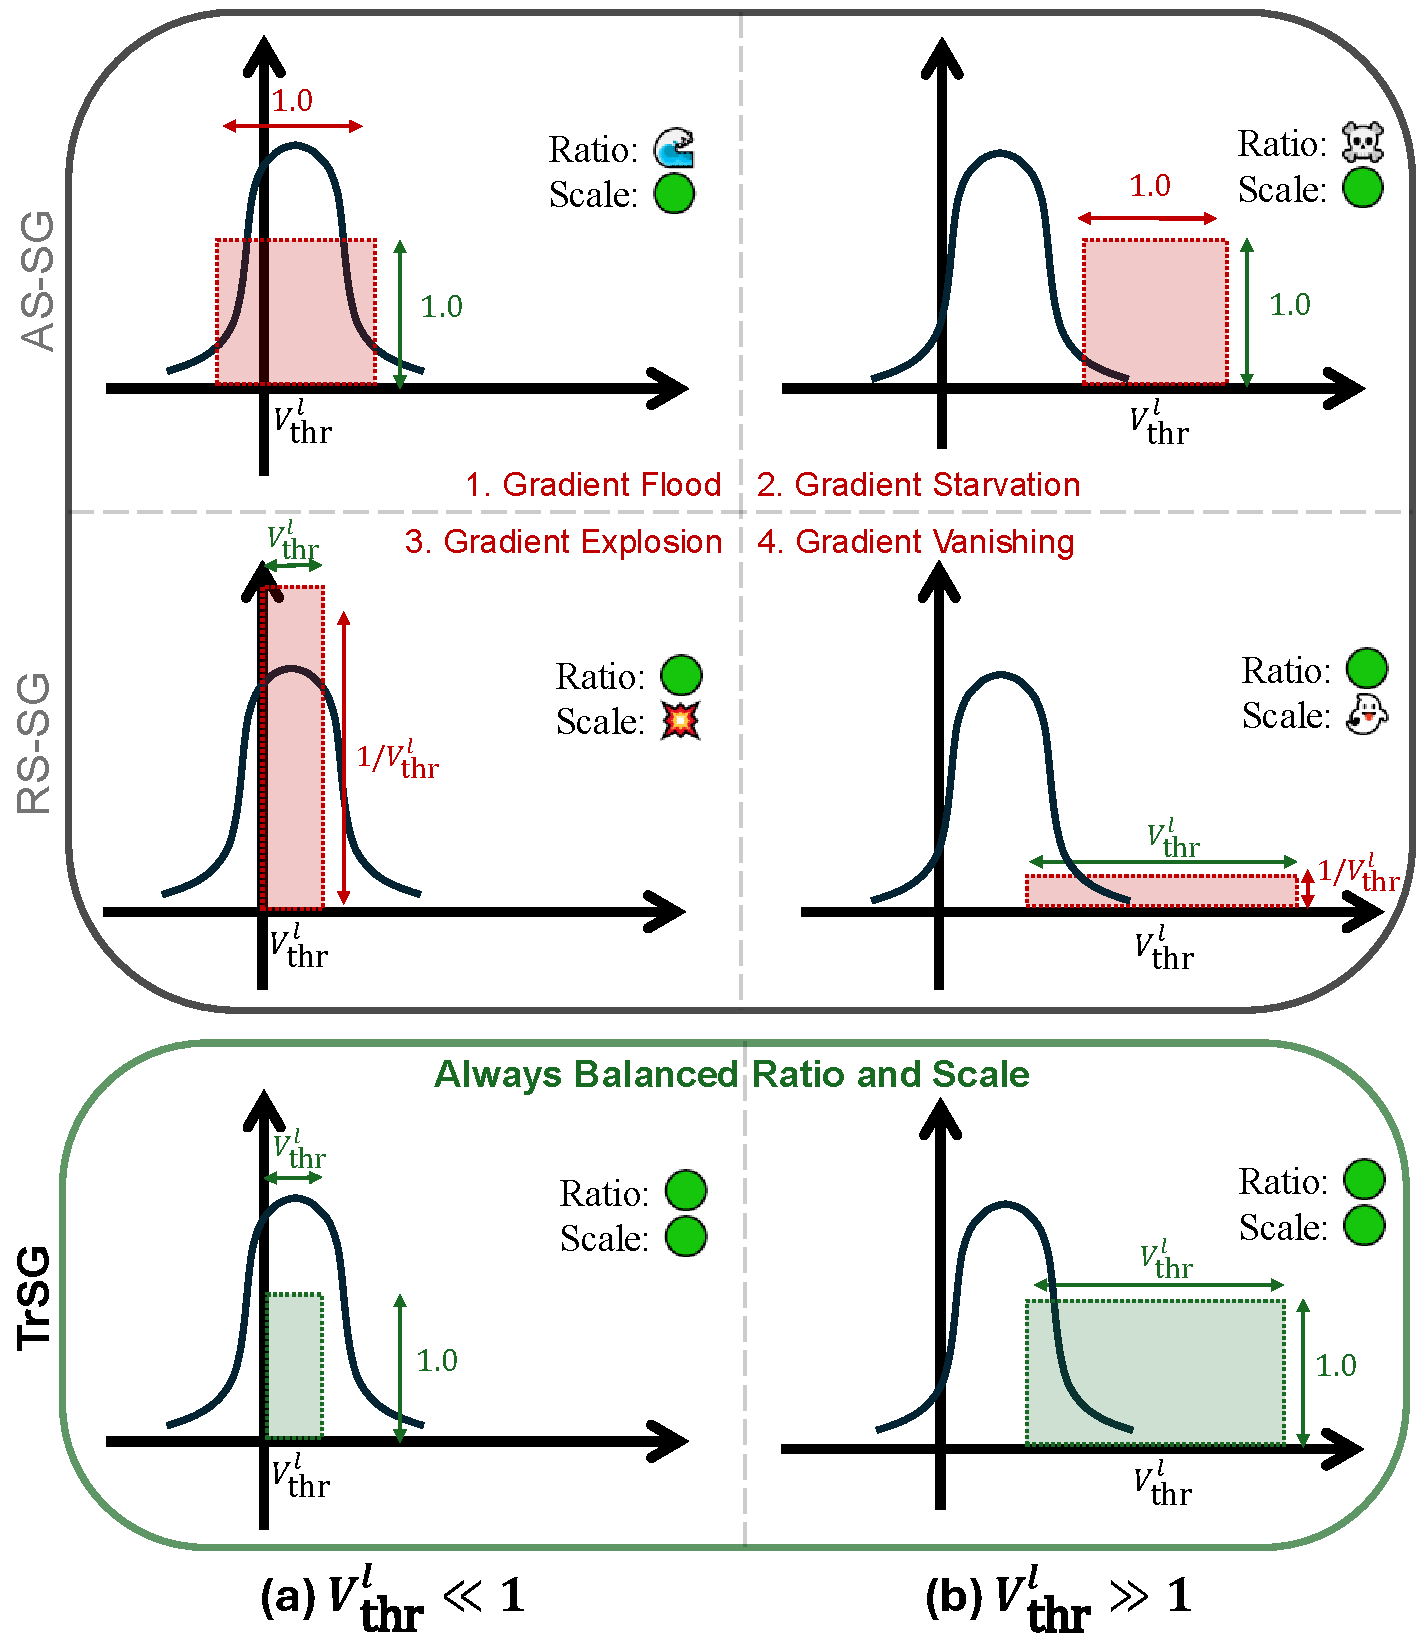
\includegraphics[width=0.99\linewidth]{fig/second_main.pdf}
    \caption{\textbf{AS-SG vs. RS-SG vs. TrSG with a rectangular surrogate gradient ($\gamma=1$).}
    The curve depicts the membrane potential distribution, while the colored boxes represent the surrogate gradient region: the horizontal span indicates the active gradient window, and the vertical extent indicates its magnitude. Panels (a) and (b) compare the behaviors when the threshold is small ($V_{\text{thr}}^{l}\!\ll\!1$) and large ($V_{\text{thr}}^{l}\!\gg\!1$), respectively. \emph{AS-SG} uses a fixed window of width $\gamma$, which leads to \textit{gradient flood} or \textit{starvation}. \emph{RS-SG} normalizes the window by $V_{\text{thr}}^{l}$ but scales the magnitude as $1/V_{\text{thr}}^{l}$, causing \textit{explosion} or \textit{vanishing}. \textbf{TrSG} multiplies the threshold forward during training, canceling the $1/V_{\text{thr}}^{l}$ factor and keeping both window and magnitude balanced across thresholds.}
    \label{fig:second_main}
\end{figure}

Surrogate Gradient (SG)~\cite{wu:2018} enables gradient-based optimization of SNNs by replacing the non-differentiable spiking function with a differentiable surrogate near the threshold. This allows effective gradient descent in SNNs, often improving performance in early timesteps. However, our analysis shows that SG used for internal neuronal parameters~\cite{fang:2021,wang:2022,rathi:2023}, particularly \(V_{\text{thr}}\), makes training highly sensitive to the \emph{scale} of \(V_{\text{thr}}\). While careful tuning can yield strong accuracy, this dependency exposes a fundamental limitation of current SG-based training.

In this section, we identify, \emph{to our knowledge for the first time}, that prior SG designs exhibit strong sensitivity of gradient flow to \(V_{\text{thr}}\). To address this, we introduce \textbf{TrSG (Threshold-robust SG)}, which maintains stable gradients regardless of the threshold value. TrSG is simple to implement, adds negligible overhead, and is compatible with a wide range of surrogate functions.

\subsection{Background: Surrogate Gradient Descent}
\label{sec:background_srgd}

As in Eq.~\ref{eq:lif_discrete_firing}, an LIF neuron emits a spike when the membrane potential crosses the threshold. Let \(H(x)\) denote the Heaviside step. Then the spike can be written as
\[
S^l[t] \;=\; H\!\bigl(x(M^l[t],V^l_{\text{thr}})\bigr),
\]
where the \emph{argument} \(x(\cdot)\) encodes how the membrane potential \(M^l[t]\) and the threshold \(V^l_{\text{thr}}\) are combined (e.g., \(x=M^l[t]-V^l_{\text{thr}}\)). 
Because \(H(\cdot)\) is non-differentiable and \(H'(\cdot)\) is a Dirac delta function, SG training replaces \(H\) with a smooth surrogate \(f\) whose derivative locally mimics \(H'\):
\[
H'(x)\;\approx\; f'(x)\quad\text{near }x=0.
\]
Applying the chain rule to the spike yields the working gradient used in training,
\begin{equation}
\label{eq:def_of_srgd}
\frac{\partial S^l[t]}{\partial M^l[t]}
\;=\;
H'\!\bigl(x\bigr)\,\frac{\partial x}{\partial M^l[t]}
\;\approx\;
f'\!\bigl(x\bigr)\,\frac{\partial x}{\partial M^l[t]},
\end{equation}
so the \emph{choice of \(x(\cdot)\)} is crucial—especially when \(V^l_{\text{thr}}\) is learnable—because it determines both the active region of nonzero gradients and the scaling of their magnitudes.

Upon reviewing the literature, SG-based methods fall into two families according to how they define \(x(M^l[t],V^l_{\text{thr}})\): \emph{Absolute-Scale SG (AS-SG)} and \emph{Relative-Scale SG (RS-SG)}. This distinction becomes significant once the threshold is trained.

\subsection{AS-SG vs. RS-SG}
\label{sec:type1_type2}

To make the scaling effects explicit, we analyze a representative surrogate with a rectangular derivative
\[
f'(x) \;=\; \frac{1}{\gamma}\,\mathds{1}\!\Bigl(|x|<\tfrac{\gamma}{2}\Bigr),
\]
where $\gamma>0$ controls the width of the region where gradients flow. The phenomena we highlight are \emph{not} specific to this choice; any surrogate exhibits the same issues.

For a better illustration, Fig.~\ref{fig:second_main} visualizes a membrane potential distribution under two different threshold scales: small ($V_{\text{thr}}^{l}\!\ll\!1$) and large ($V_{\text{thr}}^{l}\!\gg\!1$).

\paragraph{1.\;AS-SG: Absolute-Scale Surrogate Gradient.}
Many works~\cite{zheng:2021, deng:2022, fang:2021, wang:2022} take
\begin{equation}
\label{eq:abs_diff_x}
x \;=\; M^l[t] - V^l_{\text{thr}},
\end{equation}
which gives
\begin{equation}
\label{eq:abs_diff_grad}
f'\!\bigl(M^l[t]-V^l_{\text{thr}}\bigr)
\;=\;
\frac{1}{\gamma}\,\mathds{1}\!\Bigl(\bigl|M^l[t]-V^l_{\text{thr}}\bigr|<\tfrac{\gamma}{2}\Bigr),
\end{equation}
and thus
\begin{equation}
\label{eq:abs_diff_sgrad}
\frac{\partial S^l[t]}{\partial M^l[t]}
\;\approx\;
f'\!\bigl(M^l[t]-V^l_{\text{thr}}\bigr).
\end{equation}
Here the active window \(\{M^l[t]\in(V^l_{\text{thr}}-\tfrac{\gamma}{2},\,V^l_{\text{thr}}+\tfrac{\gamma}{2})\}\) has a \emph{fixed} width \(\gamma\), and the magnitude is fixed, independent of \(V^l_{\text{thr}}\). When the \(V^l_{\text{thr}}\) is small, the window becomes excessively wide relative to the membrane potential spread, so gradients keep flowing even far from the true firing boundary (\emph{gradient flood}). Conversely, when the \(V^l_{\text{thr}}\) is large, the fixed-width window covers only a tiny fraction of the distribution, and most gradients vanish (\emph{gradient starvation}). 

\paragraph{2.\;RS-SG: Relative-Scale Surrogate Gradient.}
Other works normalize by the threshold; either by \(\gamma=V^l_{\text{thr}}\)~\cite{meng:2023} or by defining
\(
x \;=\; \frac{M^l[t]}{V^l_{\text{thr}}} - 1
\)
as in~\cite{rathi:2023}. In this case,
\begin{equation}
\label{eq:rel_diff_grad}
f'\!\Bigl(\tfrac{M^l[t]}{V^l_{\text{thr}}}-1\Bigr)
\;=\;
\frac{1}{\gamma}\,\mathds{1}\!\Bigl(\Bigl|\tfrac{M^l[t]}{V^l_{\text{thr}}}-1\Bigr|<\tfrac{\gamma}{2}\Bigr),
\end{equation}
so the active window \(\{M^l[t]\in((1-\tfrac{\gamma}{2})V^l_{\text{thr}},\,(1+\tfrac{\gamma}{2})V^l_{\text{thr}})\}\) scales with \(V^l_{\text{thr}}\). 
However, the chain rule introduces a sensitivity of the gradient magnitude to the threshold:
\begin{equation}
\label{eq:rel_diff_sgrad}
\frac{\partial S^l[t]}{\partial M^l[t]}
\;\approx\;
\frac{1}{V^l_{\text{thr}}}\,
f'\!\Bigl(\tfrac{M^l[t]}{V^l_{\text{thr}}}-1\Bigr).
\end{equation}
Thus, small thresholds amplify gradients excessively (\emph{gradient explosion}), whereas large thresholds suppress them severely (\emph{gradient vanishing}). 

\subsection{Threshold-robust Surrogate Gradient}
\label{sec:ta_srgd}

We propose \textbf{TrSG}, a simple modification that preserves the desirable \emph{relative} window while canceling the problematic \(1/V^l_{\text{thr}}\) factor in the gradient. During training we (i) keep the relative-scale argument,
\[
x \;=\; \frac{M^l[t]}{V^l_{\text{thr}}} - 1,
\]
and (ii) multiply the spike by the threshold on the forward path:
\begin{equation}
\label{eq:ta_srgd_core}
O^l[t] \;=\; V^l_{\text{thr}}\cdot S^l[t].
\end{equation}
Then,
\begin{equation}
\label{eq:ta_srgd_chainrule}
\frac{\partial O^l[t]}{\partial M^l[t]}
\;=\;
V^l_{\text{thr}}\;\frac{\partial S^l[t]}{\partial M^l[t]}
\;\approx\;
V^l_{\text{thr}}\cdot
\Bigl(\frac{1}{V^l_{\text{thr}}} f'(x)\Bigr)
\;=\;
f'(x),
\end{equation}
so the gradient magnitude becomes \emph{threshold-invariant} while the active window still adapts with \(V^l_{\text{thr}}\). 

\textbf{Inference remains binary.} The scaling is training-only: at test time we revert to \(S^l[t]\in\{0,1\}\) and absorb \(V^l_{\text{thr}}\) into the next layer via a simple rescaling \(W^{l+1}_{l}\leftarrow V^l_{\text{thr}}\,W^{l+1}_{l}\). 

In summary, \textbf{TrSG} unifies a relative-scale argument with threshold multiplication on the forward path, ensuring stable gradients across thresholds. This design eliminates the flood/starvation issue of AS-SG and the vanish/explode problem of RS-SG, as further demonstrated in \cref{subsec:how_trsg_impacts_training}.
